% Claude Sonnet started LateX/Tikz with
% Please make a Latex / TikZ artfeact which has a triangle made out of 9 circles sharing edges.
% ...
% No, 3 rows on the bottom, two rows above, and one row on the top.
% ...
% Great, now make 6 of them on an A4 sheet, with bold edges.
%   & then direct edits to the LaTeX

% https://nrich.maths.org/problems/find-difference

\documentclass[a4paper]{article}
\usepackage{tikz}
\usepackage[margin=1cm]{geometry}

\begin{document}
\pagestyle{empty}

\begin{center}
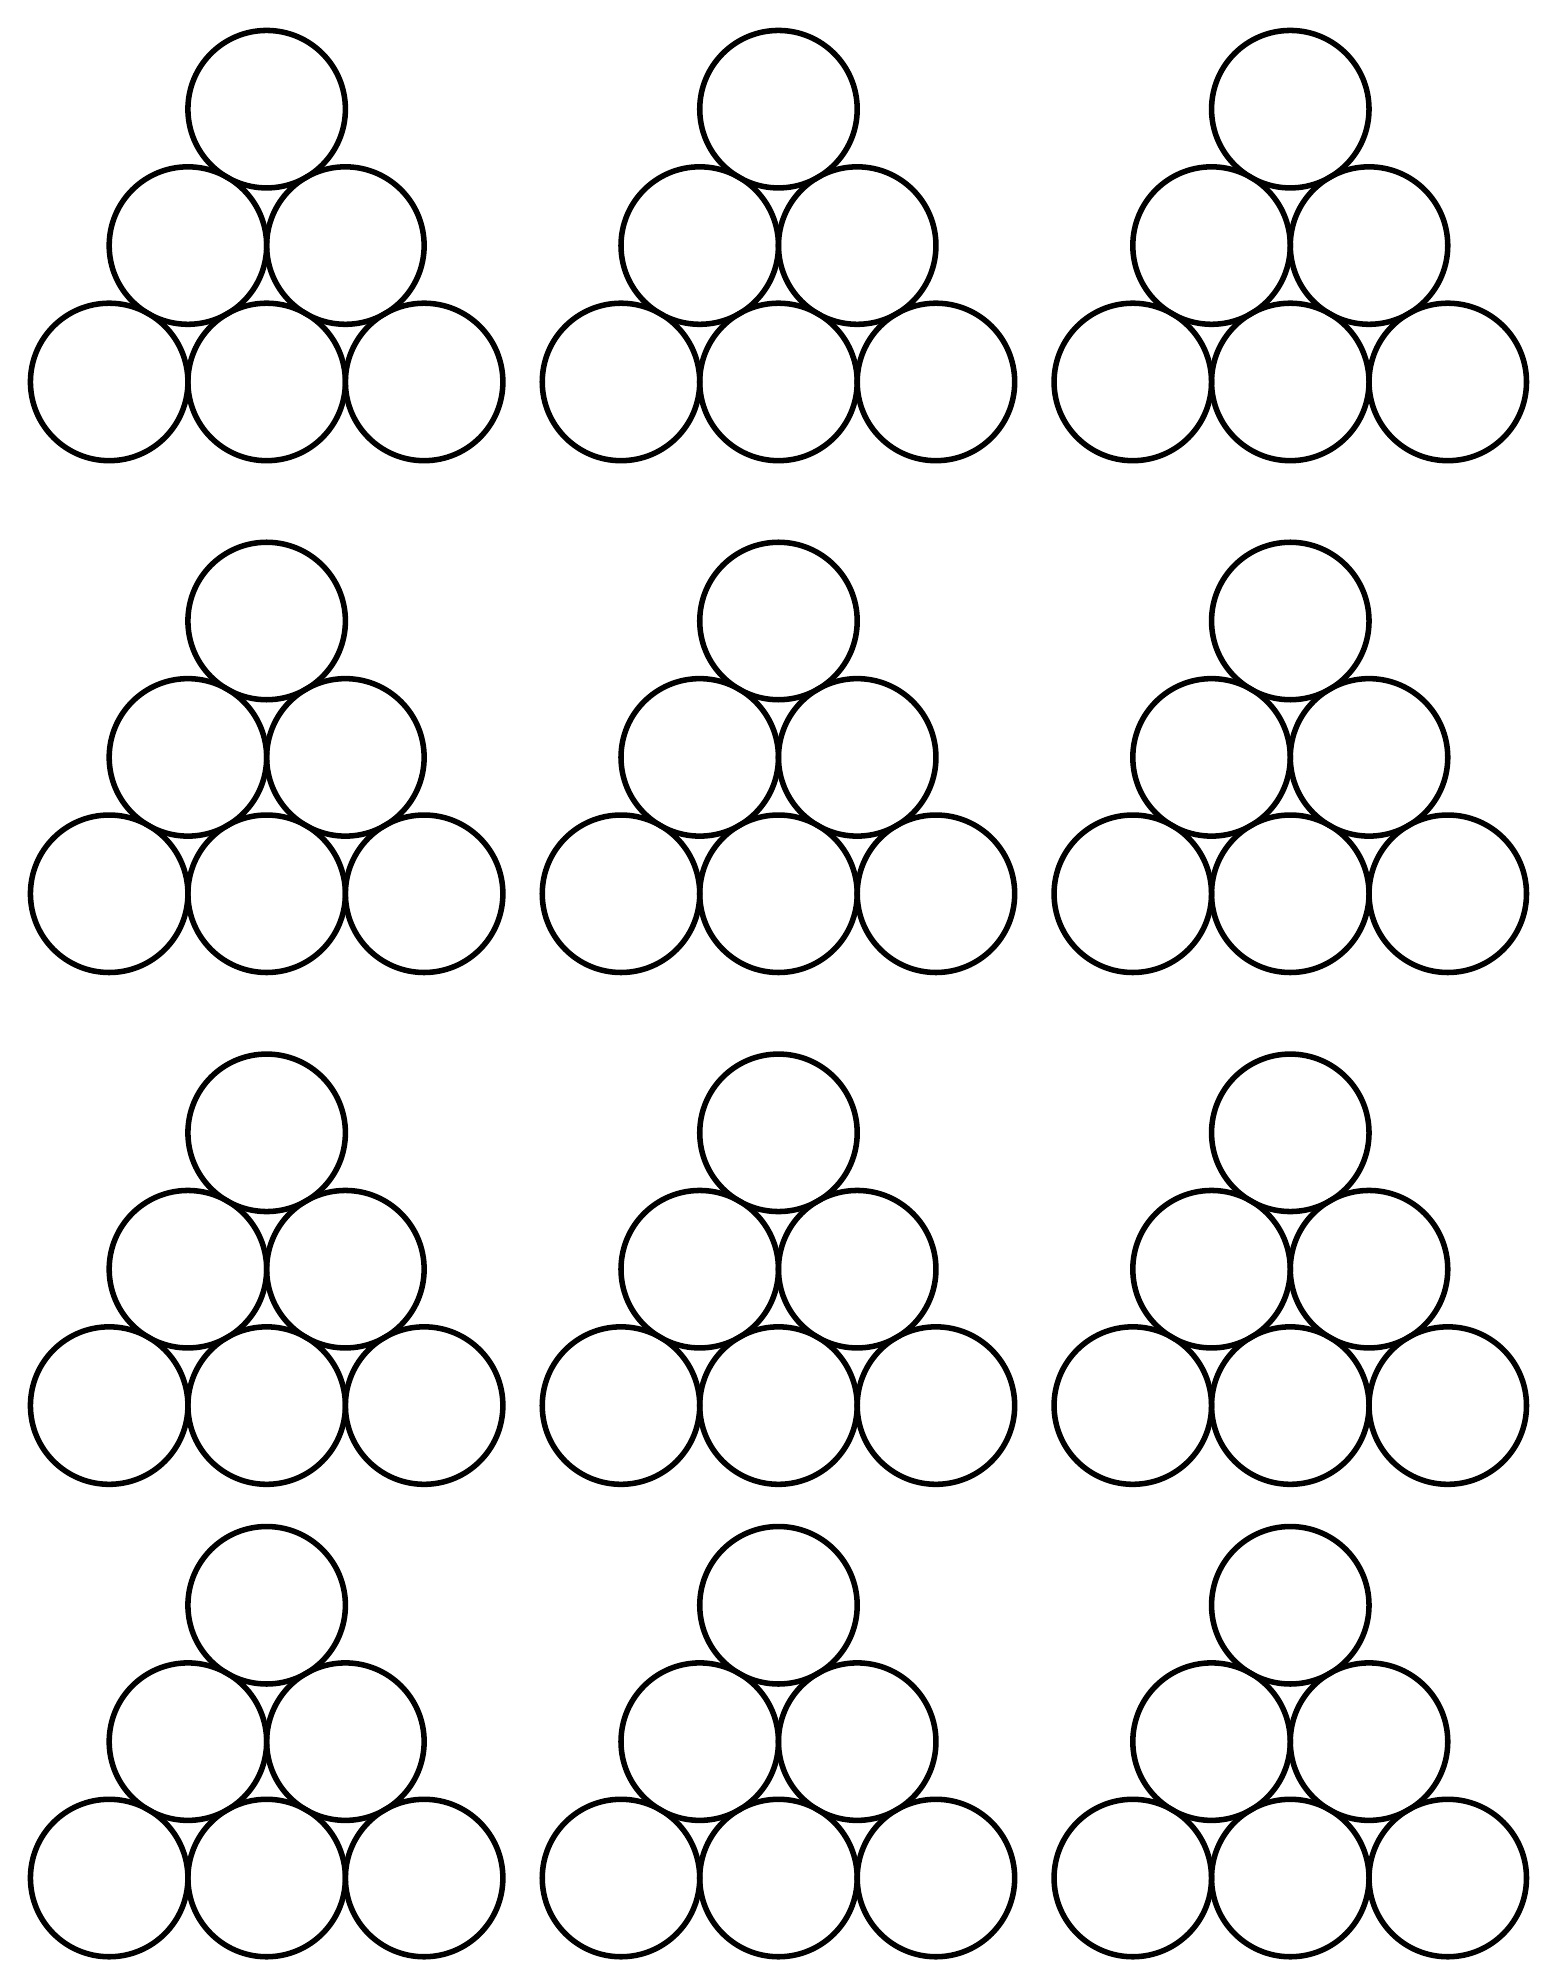
\begin{tikzpicture}[line width=2.0pt]  % Making all lines bolder

% Define the radius of circles - slightly smaller to fit 6 on page
\def\r{1.0}

% First row of 3 arrangements
\foreach \row in {-1,-7.5,-14,-20} {

\foreach \shift in {0,6.5,13} {
    % Bottom row (3 circles)
    \foreach \i in {0,1,2} {
        \draw ({2*\r*\i+\shift},{0+\row}) circle (\r);
    }
    % Middle row (2 circles)
    \foreach \i in {0,1} {
        \draw ({2*\r*\i+\r+\shift},{2*\r*sin(60)+\row}) circle (\r);
    }
    % Top row (1 circle)
    \draw ({2*\r+\shift},{4*\r*sin(60)+\row}) circle (\r);
}
}


\end{tikzpicture}
\end{center}

\end{document}